\documentclass[spanish]{article}
\usepackage[spanish]{babel} %esto es para que las ondas estn en espaol
\usepackage{url} % para la bibliografia
\usepackage{sectsty}
\usepackage{graphicx}
\usepackage{tikz}
\usepackage{verbatim}
\usepackage{listings}
\usepackage{amsfonts}
\usetikzlibrary{calc}

\usepackage[utf8x]{inputenc}

\newcommand{\sectionline}{%
  \nointerlineskip \vspace{\baselineskip}%
  \hspace{\fill}\rule{0.5\linewidth}{.7pt}\hspace{\fill}%
  \par\nointerlineskip \vspace{\baselineskip}
}

\usepackage{color}
\definecolor{dkgreen}{rgb}{0,0.6,0}
\definecolor{gray}{rgb}{0.5,0.5,0.5}
\definecolor{mauve}{rgb}{0.58,0,0.82}

\lstset{frame=tb,
  language=Python,
  aboveskip=3mm,
  belowskip=3mm,
  showstringspaces=false,
  columns=flexible,
  basicstyle={\small\ttfamily},
  numbers=none,
  numberstyle=\tiny\color{gray},
  keywordstyle=\color{blue},
  commentstyle=\color{dkgreen},
  stringstyle=\color{mauve},
  frame=none,
  breaklines=true,
  breakatwhitespace=true
  tabsize=3
}

\lstset{frame=tb,
  language=Java,
  aboveskip=3mm,
  belowskip=3mm,
  showstringspaces=false,
  columns=flexible,
  basicstyle={\small\ttfamily},
  numbers=none,
  numberstyle=\tiny\color{gray},
  keywordstyle=\color{blue},
  commentstyle=\color{dkgreen},
  stringstyle=\color{mauve},
  frame=none,
  breaklines=true,
  breakatwhitespace=true
  tabsize=3
}
%Para que los numeros de las secciones estn del lado izquierdo del margen
\makeatletter
\def\@seccntformat#1{\protect\makebox[0pt][r]{\csname
	the#1\endcsname\quad}}
\makeatother

\begin{document}

\title{Investigaci\'{o}n 2: MapReduce \linebreak
CC3008 - Sistemas Operativos Avanzados } 
\author{Carlos López (08107) y Héctor Hurtarte (08119) \\ 
Universidad del Valle de Guatemala}
\date{Octubre del 2010}
\maketitle

\begin{abstract}
  \textbf{MapReduce} es un modelo de programación para procesar datos a larga escala, diseñado para implementarse en sistemas distribuídos. Está inspirado en las funciones \textbf{Map} y \textbf{Reduce}, he de ahí su nombre. El modelo consiste en:
  \begin{itemize}
    \item Una función \textbf{map}
    \item Una función \textbf{reduce}
    \item Paralelizar las tareas y balancear la carga entre nodos, coordinado por un programa principal (``Programa master'') para procesar los datos y obtener el resultado esperado.
    \item También incluye mecanismos para tolerar fallas de nodos y también para evitar que \textit{stragglers} (nodos que se atrasan en realizar sus tareas) retrasen el resultado.
  \end{itemize}
\end{abstract}

\section{Introducción}
La programación funcional nació con el lenguaje Lisp, diseñado por John McCarthy a finales de los años 50 y basado completamente en el cálculo lambda de Alonzo Church \cite{HistoriaLisp}. Durante años, el paradigma de la función funcional fué puramente académico y en las últimas dos decadas, ha surgido como una alternativa importante para resolver problemas en la ciencia de la computación.

Una de sus aplicaciones importantes es que si se cumplen ciertas normas -- explicadas más adelante -- se puede conseguir aplicaciones \textit{thread-safe}, es decir, que \textit{threads} puedan realizar tareas y comunicarse entre sí conrurrentemente sin que existan problemas de sincronización entre ellos. Esto es un atributo muy importante que deben mantener los sistemas distribuídos ya que en estos existen diferentes nodos que realizan \textit{mini-tareas} para realizar una operación \textit{más compleja} compartiendo datos y estructuras.

\section{Principios básicos de programación funcional y atributos}

\subsection{La función Map}
La función \textbf{Map}, como su nombre lo dice, mapea elementos de un tipo hacia otro, tal como una función matemática. Ésta generalmente está definida sobre listas pero puede actuar sobre otras estructuras e.g. Arreglos, Conjuntos o Secuencias iterables.

En un lenguaje tipíficado, la función \textbf{Map} necesita de:
\begin{itemize}
  \item Una lista de $A$'s, denotada $[A]$ en donde $A$ es un tipo.
  \item Una función $f: A \rightarrow B$
\end{itemize}

El resultado de ejecutar \textbf{Map} junto con $f$ y $[A]$, es una lista de $B$'s: $[B]$. La firma de esta función es 

\[ (A \rightarrow B) \rightarrow [A] \rightarrow [B]\]

y se lee ``Una función que toma una función que toma un $A$ para devolver un $B$ que luego toma una lista de $A$'s para devolver una lista de $B$'s''

\textbf{Ejemplos:}
\begin{itemize}
  \item En ipython:
    \lstinputlisting[language=Python]{programas-ejemplo/map.py}
\end{itemize}

\subsection{La función Reduce}
La función \textbf{Reduce}, también está definida sobre listas y su objetivo es \textit{reducir} una lista de $A's$ a un valor de tipo $B$.

En un lenguaje tipíficado, la función \textbf{Reduce} necesita de:
\begin{itemize}
  \item Al igual que Map, una lista de $A'$s para actuar sobre ella: $[A]$. 
  \item Una función binaria $f: (B,A) \rightarrow B$
\end{itemize}

El resultado de ejecutar \textbf{Reduce} sobre $[A]$ utilizando $f$ para operar los resultados de cada operación binaria desde el inicio o fin de la lista de $A$'s, es un valor de tipo $B$. Esta trata de reduci por tuplas con $f$ y siempre empieza por un lado a transversar la lista (izquierda o derecha). 

\textbf{Ejemplos:}
\begin{itemize}
  \item En ipython:
    \lstinputlisting[language=Python]{programas-ejemplo/reduce.py}
\end{itemize}

\subsection{Programación funcional en un sistema distribuído}
Habíamos hablado en la introducción sobre el rol de un lenguaje funcional en un sistema distribuído. En uno de estos lenguajes, las operaciones y sus resultados están basadas en funciones, contrario a los lenguajes comunes como Java o C++ en donde uno declara instrucciones en una forma imperativa y estas son inmediatamente computadas.

Consideremos las siguientes estructuras escritas en Java:
\lstinputlisting[language=Java]{programas-ejemplo/side-effects.java}

Podemos observar rápidamente que el programa que utilice más de un \textbf{EjecutorDeTransacciones} concurrentemente, tendrá problemas de sincronización y decimos que el programa tiene efectos secundarios (o \textit{side-effects}). En una función nunca puede haber este tipo de problemas ya que es libre de \textit{side-effects}: una función que su valor de retorno dependa únicamente de sus argumentos, no puede tener problemas de sincronización con otras estructuras o funciones, ya que sus variables están limitadas a ser utilizadas sólamente por la función que las necesita, a estas variables les llamamos \textbf{bounded variables}.

En conclusión, las funciones mantienen siempre un estado y donde todas las variables son inmutables, es decir, que no cambian de valor. Por lo tanto, pensando en \textit{thread-safety}, podemos decir que la programación funcional \textbf{promueve la exclusión mutua} en sistemas distribuídos.

\section{Implementación}
Los detalles sobre la implementación del modelo de MapReduce dependen del entorno. Para el presente trabajo considerese un entorno como el siguiente \cite{MapReduceGoogle}:
\begin{itemize}
   	\item Muchas computadoras con procesador dual x86, Linux y 2-4 GB de memoria o similar.
   	\item Red con conexión de 100 Mbps a 1 Gbps.
   	\item \textit{Clusters} con cientos o miles de computadoras (propenso a fallas).
   	\item \textit{Filesystem} distribuído con replicación (GFS).
   	\item Usuarios que presentan \textit{jobs} a calendarizador.
\end{itemize}

\subsection{Ejecuci\'{o}n}
	Las invocaciones de \textit{Map} se distribuyen entre múltiples equipos particionando automáticamente el \textit{input} en un conjunto de \textit{M} \textit{splits}. Estos \textit{splits} pueden ser procesados en paralelo por diferentes equipos. Las invocaciones de \textit{Reduce} se distribuyen particionando las llaves intermedias en \textit{R} trozos usando una función de partición. Este es el flujo de una operación de MapReduce en la presente implementación \cite{MapReduceGoogle}: 
\begin{center}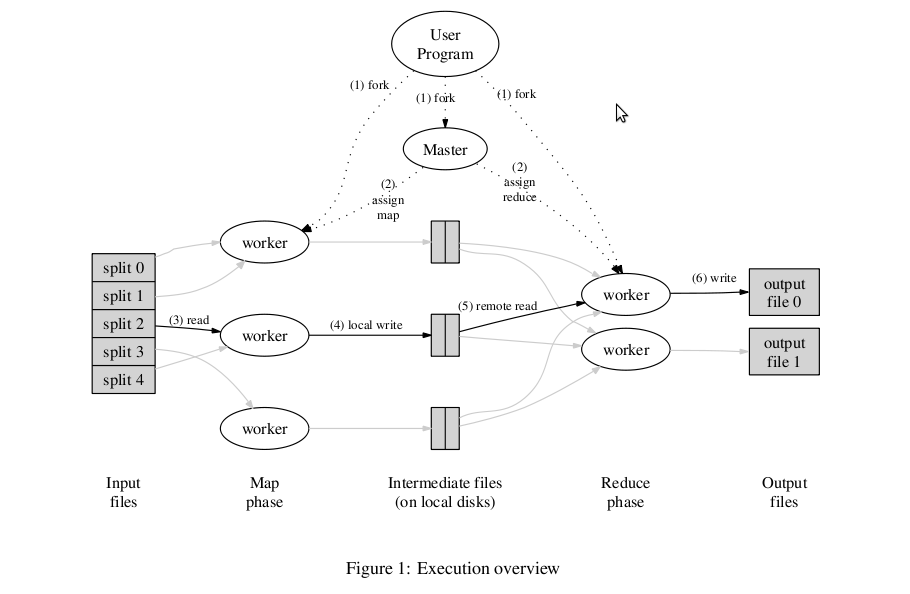
\includegraphics[width=13.5cm]{imagenes/ExecutionOverview.png}\end{center}
\begin{enumerate}
	\item La librer\'{i}a de MapReduce en el \textit{user program} primero divide el \textit{input} en \textit{M} trozos de 16 a 64 MB. Luego arranca varias copias del programa en un \textit{cluster} de m\'{a}quinas.
	\item Una de las copias del programa se asigna como \textit{master} y el resto son trabajadores. Se asignan \textit{M} tareas \textit{map} y \textit{R} tareas \textit{reduce}. El \textit{master} escoge trabajadores inactivos y asigna tareas.
	\item Un trabajador a quien se le asigna una tarea \textit{map} obtiene el contenido del \textit{input split} correspondiente. Luego \textit{parsea} pares llave/valor y los proporciona a la función \textit{map} definida por el usuario. Los pares intermedios llave/valor producidos por la función se almacenan en memoria \textit{buffer}.
	\item Periodicamente, los pares en \textit{buffer} se escriben a discos locales, particionados en \textit{R} regiones por una funci\'{o}n de partici\'{o}n. La posici\'{o}n de estos pares luego de moverse a discos locales se env\'{i}an a \textit{master}. 
	\item Cuando a un trabajador de \textit{reduce} se le notifica sobre estas posiciones, utiliza llamadas a procedimientos remotos para leer esta \textit{data}. Luego de leer toda la \textit{data} intermedia la ordena y agrupa seg\'{u}n la llave intermedia. 
	\item Este trabajador itera sobre la \textit{data} intermedia ordenada y para cada llave intermedia \'{u}nica pasa la llave y su correspondiente conjunto de valores intermedios a la funci\'{o}n \textit{reduce} del usuario. El \textit{output} se añade al archivo final de \textit{output} para esta partición de \textit{reduce}.
	\item Cuando todas las tareas han sido completadas, el \textit{master} devuelve el control al \textit{user program}. 
\end{enumerate}
\subsection{Estructuras y parámetros}
	Para cada tarea \textit{map} y \textit{reduce}, el proces \textit{master} almacena el estado de la tarea (\textit{idle}, \textit{in-progress} o \textit{completed}) y la identidad de la máquina trabajadora.
	
	El proceso \textit{master} es el conducto por el que la posición de las regiones de archivos intermedios se propagan de tareas \textit{map} a \textit{reduce}. Por lo tanto, para cada tarea \textit{map} completada, el \textit{master} almacena la posición y tamaño de las \textit{R} regiones intermedias producidas por \textit{map}. Las actualizaciones a estas posiciones y tamaños se reciben a medida que se completan las tareas \textit{map} y se añaden incrementalmente a trabajadores con procesos \textit{reduce} en estado \textit{in-progress}.
\subsection{Balanceo, granularidad y complejidad}
	La fase de \textit{map} se subdivide en \textit{M} trozos y la de reduce en \textit{R}. Idealmente \textit{M} y \textit{R} serán mucho más grandes que la cantidad de máquinas disponibles de forma que muchos trabajdores lleven a cabo muchas tareas diferentes. Esto mejora el balanceo de carga dinámico dado que cada trabajador tendrá aproximadamente el mismo número de tareas. De la misma forma, al fallar un trabajador, sus tareas podrán repartirse mejor entre los demás. 
	
	Las limitantes a los tamaños de \textit{M} y \textit{R} se establecen dado que el proceso \textit{master} debe efectuar \textit{O(M+R)} decisiones de calendarización y mantener \textit{O(M$\cdot$R)} estados en memoria. Adem\'{a}s de eso, el usuario suele limitar \textit{R} porque el \textit{output} de cada tarea \textit{reduce} termina en un archivo diferente. 
	
	En la pr\'{a}ctica \textit{M} suele elgirse de forma que cada tarea individual sea de 16 a 64 MB de \textit{input data} y \textit{R} de forma que sea un m\'{u}ltiplo del n\'{u}mero de trabajadores. 

\subsection{Tolerancia a fallas}
	El modelo de MapReduce está diseñado para procesar grandes cantidades de \textit{data} en cientos o miles de equipos, por lo que la tolerancia a fallas debe ser robusta. Se consideran los siguientes casos:
    \begin{itemize}
    	\item \textbf{Trabajador}: El \textit{master} hace \textit{ping} a cada trabajador periódicamente. Si no se recibe respuesta en cierto tiempo, el \textit{master} marca al trabajador como fallido. Cualquier tarea \textit{map} completada se reinicia dado que su \textit{output} está almacenado en discos locales y por tanto es inaccesible. Cualquier tarea \textit{map} o \textit{reduce} en progreso también se reinicia. Cuando una tarea \textit{map} pasa de un equipo a otro (por fallo) todos los trabajadores que ejecutan \textit{reduce} son notificados e inician a leer data del nuevo \textit{map}. 
    	
    	La fiabilidad de este sistema se probó extendamente durante una operación de mantenimiento en un \textit{cluster} de 1,800 servidores. Se desconectaron grupos de 80 equipos a la vez. Los procesos corrieron un poco lentos pero se completaron \cite{MapReduceNews}.
    	\item \textbf{\textit{Master}}: El master escribe periódicamente \textit{checkpoints} a partir de los cuales es fácil crear una nueva copia en caso que falle. Sin embargo, dado que solo hay un \textit{master} por cada ejecución de MapReduce, es poco probable que falle; por lo tanto la implementación actual de MapReduce aborta cuando falla el \textit{master}. Los clientes pueden revisar esta condición y reintentar la operación a voluntad.
\end{itemize}
El proceso confía en \textit{commits} atómicos de los \textit{outputs} de \textit{map} y \textit{reduce}. Cada tarea en proceso escribe su \textit{output} a archivos privatos temproales. Una tarea \textit{reduce} produce un solo archivo, y una \textit{map} produce \textit{R}. Cuando un proceso \textit{map} termina, el trabajador envía un mensaje al \textit{master} e incluye el nombre de los \textit{R} archivos temporales.

Cuando una tarea \textit{reduce} se completa, el trabajador automáticamente renombra su archivo temporal de \textit{output} con el nombre del archivo final. Si la misma tarea \textit{reduce} se ejecuta por varias máquinas, se invocaran múltiples renombramientos para el mismo \textit{output file}. Es por esto que se confía en la atomicidad del proceso de renombrar de parte del sistema operativo. 

\subsection{Combatiendo \textit{stragglers}: Tareas de backup}
Una de las causas del prolongamiento del tiempo en completar una operación de MapReduce son los \textit{stragglers} (rezagados): máquinas a las que les toma una cantidad inusual de tiempo completar una de las últimas tareas de \textit{map} o \textit{reduce} en la operación. Las causas de los \textit{stragglers} abarcan, por ejemplo, m\'{a}quinas con discos duros defectuosos que presentan errores corregibles pero relentizan el performance de 30 a 1 MB/s, o bien que el sistema de calendarización del cluster les imponga otras tareas o incluso que por problemas de inicializaci\'{o}n no tengan habilitada la \textit{cache} del procesador. 

El mecanismo general para atacar este problema involucra que, cuando la operaci\'{o}n MapReduce est\'{a} por completarse, el \textit{master} calendariza operaciones \textit{backup} de las tareas \textit{in-progress}. La tarea se marca como finalizada cuando cualquiera de los trabajadores completa la asignaci\'{o}n. El mecanismo se ha afinado de forma que solo consuma m\'{a}s recursos en un bajo porcentaje. Se ha encontrado que este proceso reduce el tiempo para completar operaciones voluminosas. Por ejemplo, al programa de ejemplo de la secci\'{o}n 5.3 de \cite{MapReduceGoogle} le toma 44\% m\'{a}s tiempo terminar cuando este mecanismo est\'{a} deshabilitado.

\subsection{Aplicaciones}
Existe una grande variedad de procesos que se pueden computar con este modelo, Google ha logrado ponerlo en práctica en los siguientes escenarios:
\begin{enumerate}
\item Grep distribuído: Analiza un conjunto de archivos en diferentes nodos junto con una expresión regular y lista los que contengan el patrón. \cite{GrepDistribuido}
  \begin{itemize}
    \item Función Map: $f: (Offset del archivo, linea) \rightarrow Either[Nil,(Linea,1)$, es decir, toma una pareja ordenada (Archivo, linea) y responde con una lista vacía ($Nil$) o una pareja ordenada $(linea,1)$ si concuerda con el patrón.
    \item Función Reduce: $r: (linea,[1,1,1...1]) \rightarrow (linea,n)$ en donde $n$ es la cantidad de 1's que aparecen en la entrada de la función
  \end{itemize}
  
  \item PageRank, programa implementado por Google para \textit{rankear} cualquier tipo de documentos, principalmente URL's. \cite{GrepDistribuido}
  \begin{itemize}
    \item Empieza con un par ordenado $(URL,[URL])$ en donde la llave es una URL cualquiera y $[URL]$ es la lista de links contnidas en la llave.
    \item Utiliza una función que mapea a $(URL,(PageRanking,[URL_2]))$
    \item Para cada $u \in [URL_2]$, retorna tanto $u,(PR,[URL_2)$ como $(u,[URL_4])$.
    \item La función reduce recibe $(URL,[URL])$ y varios pares de la forma $(URL,valor)$ y calcula $(URL,(nuevoPageRank,[URL]))$
  \end{itemize}

  \item Machine Learning
  \item Statistical machine translation
\end{enumerate}
%kmels

\addcontentsline{toc}{chapter}{Bibliografía}
\begin{thebibliography}{99}
%********************************************
% kmels
%********************************************
\bibitem{HistoriaLisp} \textit{History of Lisp, John McCarthy, Artificial Intelligenge Laboratory, Stanford University, 12 February 1979, \url{http://www-formal.stanford.edu/jmc/history/lisp/lisp.html} }
\bibitem{GrepDistribuido} \textit{Applications of MapReduce, Distributed Computing Systems, CS 4513, Department of Computer Science, Worcester Polythechnic Institute, \url{http://web.cs.wpi.edu/~cs4513/d08/OtherStuff/MapReduce-TeamC.ppt}}



%********************************************
% hector
%********************************************
\bibitem{MapReduceGoogle} Dean, J. y Ghemawat S. \textit{MapReduce: Simplified Data Processing on Large Clusters}. Google, Inc. 2004.
\bibitem{MapReduceWikipedia} Wikipedia Foundation, Inc. \textit{MapReduce}. Consultado 8 de Noviembre de 2010. Sitio web: \url{http://en.wikipedia.org/wiki/MapReduce}
\bibitem{MapReduceEdu} Bisciglia, C. et al. \textit{MapReduce Theory and Implementation}. Distributed computer seminar. Google, Inc. Consultado 8 de Noviembre de 2010. Sitio web: \url{http://code.google.com/edu/submissions/mapreduce/llm3-mapreduce.ppt} 
\bibitem{MapReduceNews} Shankland, S. \textit{Google spotlights data center inner working}. CNet News. Consultado 8 de Noviembre de 2010: Sitio web: \url{http://news.cnet.com/8301-10784_3-9955184-7.html}. 


\end{thebibliography}
\end{document}
